\documentclass[10pt,aspectratio=169]{beamer}

\usetheme[progressbar=frametitle]{metropolis}

\title{Mathematische Aspekte des maschinellen Lernens}
\subtitle{Approximationstheorie}
\date{19.11.2021}
\author{Pavel Zwerschke}
\institute{Karlsruher Institut für Technologie}
\titlegraphic{\hfill
\includegraphics[height=1.5cm]{logos/kit-de}}

% BibTeX setup
\usepackage[backend=bibtex, bibstyle=alphabetic, citestyle=alphabetic]{biblatex}
\bibliography{references}

% \usepackage[english]{babel} % English
\usepackage[ngerman]{babel} % German

% Standard packages for math-related things.
\usepackage{amsmath}
\usepackage{amssymb}
\usepackage{amsthm}
\usepackage{mathtools}

\usepackage{graphicx} % to include graphics with \includegraphics[options]{imagefile}
\definecolor{lightblue}{RGB}{189,216,238}

\theoremstyle{plain} % Usual style for theorems, etc.

\setbeamertemplate{theorems}[numbered]

% All numbered with the same counter (theorem).
%\newtheorem{theorem}{Theorem}[section] % This uses numbering SECTION.COUNT instead of COUNT. Useful in longer documents.
%\newtheorem{theorem}{Satz} % Number linearly (no SECTION prefix).
% Usage: \newtheorem{environmentname}[counter]{displayedtext}
\newtheorem{proposition}[theorem]{Proposition}
% \newtheorem{lemma}[theorem]{Lemma}
\newtheorem{satz}[theorem]{Satz}
\newtheorem{korollar}[theorem]{Korollar}
\newtheorem*{lemma*}{Lemma} % not numbered.
\newtheorem*{satz*}{Satz} % not numbered.

% \theoremstyle{definition} % Usual style definitions.
% \newtheorem{definition}[theorem]{Definition}

\theoremstyle{remark} % Usual style definitions.
\newtheorem{remark}[theorem]{Remark}

\newcommand{\N}{\mathbb{N}} % blackboard bold N for natural numbers
\newcommand{\R}{\mathbb{R}} % blackboard bold R for real numbers
\newcommand{\Z}{\mathbb{Z}} % blackboard bold Z for integers

\newcommand{\set}[1]{\{#1\}}
\newcommand{\norm}[1]{\|#1\|}

\begin{document}

\maketitle

\begin{frame}{Inhaltsverzeichnis}
    \setbeamertemplate{section in toc}[sections numbered]
    \tableofcontents%[hideallsubsections]
\end{frame}

\section{Definitionen}

\begin{frame}{ReLU Netzwerk}
    \begin{definition}[ReLU Netzwerk]
        Sei \(L \in \N\) und \(N_0, N_1, \ldots, N_L \in \N\). Ein 
        \textit{ReLU neuronales Netz} \(\Phi\) ist eine Abbildung 
        \(\Phi: \R^{N_0} \rightarrow \R^{N_L}\), die durch 
        \[ \Phi = \begin{cases}
            W_1, & L = 1, \\
            W_L \circ \rho \circ \cdots \circ \rho \circ W_1, & L \geq 2
        \end{cases} \]
        gegeben ist. Hierbei ist für \(l\in \set{1,\ldots, L}\) \(W_l : \R^{N_{l-1}} \rightarrow \R^{N_l}, W_l(x) = A_l x + b_l\) 
        die jeweilige affine Transformation und \(\rho: \R \rightarrow \R\), \(\rho(x) := \max\set{0, x}\) 
        die ReLU-Funktion (komponentenweise).

        Die Menge aller ReLU Netzwerke mit Input-Dimension \(N_0 = d\) und Output-Dimension \(N_L = d'\) 
        definieren wir als \(\mathcal{N}_{d,d'}\).
    \end{definition}
\end{frame}

\begin{frame}{Eigenschaften eines ReLU Netzwerks}
    \begin{definition}[Eigenschaften eines ReLU Netzwerks]
        \begin{description}
            \item[Konnektivität] \(\mathcal{M}(\Phi)\) ist die Anzahl der nicht null Einträge in den Matrizen \(A_1, \ldots, A_L\) 
            sowie Bias Vektoren \(b_1, \ldots, b_L\),
            \item[Tiefe] \(\mathcal{L}(\Phi) := L\),
            \item[Breite] \(\mathcal{W}(\Phi) := \max_{l=0,\ldots, L} N_l\),
            \item[Gewicht] \(\mathcal{B}(\Phi) := \max_{l=1,\ldots, L} \max\set{\norm{A_l}_\infty, \norm{b_l}_\infty}\).
        \end{description}
    \end{definition}
\end{frame}

\begin{frame}{Komposition von ReLU Netzwerken}
    \begin{lemma}
        Seien \(d_1\), \(d_2\), \(d_3 \in \N\), \(\Phi_1 \in \mathcal{N}_{d_1, d_2}\), \(\Phi_2 \in \mathcal{N}_{d_2, d_3}\). Dann existiert ein 
        Netzwerk \(\Psi \in \mathcal{N}_{d_1, d_3}\) mit \(\mathcal{L}(\Psi) = \mathcal{L}(\Phi_1) + \mathcal{L}(\Phi_2)\), 
        \(\mathcal{M}(\Psi) \leq 2 \mathcal{M}(\Phi_1) + 2\mathcal{M}(\Phi_2)\), \(\mathcal{W}(\Psi) \leq 
        \max\set{2d_2, \mathcal{W}(\Phi_1), \mathcal{W}(\Phi_2)}\), \(\mathcal{B}(\Psi) = \max\set{\mathcal{B}(\Phi_1), \mathcal{B}(\Phi_2)}\) 
        sowie
        \[ \Psi(x) = (\Phi_2 \circ \Phi_1)(x) = \Phi_2(\Phi_1(x)) \ \ \forall x\in \R^{d_1}. \]
    \end{lemma}
\end{frame}

\newcommand{\mynode}[4]{
    \node[ReceptorNode] (circ-#1-#2) at (#3, #4) {};
}
\newcommand{\connect}[4]{
    \draw[Connection] (circ-#1-#2) -- (circ-#3-#4);
}
\begin{frame}{Komposition von ReLU Netzwerken}
    \centering
    \begin{tikzpicture}
    \tikzset{ReceptorNode/.style={circle, draw=black, fill=lightblue, thick, inner sep=2pt, minimum size=20pt}}
    \tikzset{Connection/.style={->, line width=0.25mm}}
    
    \foreach \n in {0,...,4}{\mynode{0}{\n}{0}{\n}}
    \foreach \n in {0,...,3}{\mynode{1}{\n}{3}{\n+0.5}}
    \foreach \n in {0,...,4}{\mynode{2}{\n}{6}{\n}}
    \foreach \n in {0,...,4}{
        \foreach \m in {0,...,3}{
            \connect{0}{\n}{1}{\m}
        }
    }
    \foreach \n in {0,...,3}{
        \foreach \m in {0,...,4}{
            \connect{1}{\n}{2}{\m}
        }
    }
    \node at (3, 5) {\(\Phi_1\)};
    \end{tikzpicture} \qquad
    \begin{tikzpicture}
    \tikzset{ReceptorNode/.style={circle, draw=black, fill=lightblue, thick, inner sep=2pt, minimum size=20pt}}
    \tikzset{Connection/.style={->, line width=0.25mm}}
    
    \foreach \n in {0,...,4}{\mynode{0}{\n}{0}{\n}}
    \foreach \n in {0,...,1}{\mynode{1}{\n}{3}{\n+1.5}}
    \foreach \n in {0,...,4}{
        \foreach \m in {0,...,2}{
            \connect{0}{\n}{1}{\m}
        }
    }
    \node at (1.5, 5) {\(\Phi_2\)};
    \end{tikzpicture}
\end{frame}

\begin{frame}{Komposition von ReLU Netzwerken}
    \centering
    \begin{tikzpicture}
    \tikzset{ReceptorNode/.style={circle, draw=black, fill=lightblue, thick, inner sep=2pt, minimum size=20pt}}
    \tikzset{Connection/.style={->, line width=0.25mm}}
    
    \foreach \n in {0,...,4}{\mynode{0}{\n}{0}{\n}}
    \foreach \n in {0,...,3}{\mynode{1}{\n}{3}{\n+0.5}}
    \foreach \n in {0,...,4}{\mynode{2}{\n}{6}{\n}}
    \foreach \n in {0,...,1}{\mynode{3}{\n}{9}{\n+1.5}}
    \foreach \n in {0,...,4}{
        \foreach \m in {0,...,3}{
            \connect{0}{\n}{1}{\m}
        }
    }
    \foreach \n in {0,...,3}{
        \foreach \m in {0,...,4}{
            \connect{1}{\n}{2}{\m}
        }
    }
    \foreach \n in {0,...,4}{
        \foreach \m in {0,...,1}{
            \connect{2}{\n}{3}{\m}
        }
    }

    \node at (4.5, 5) {\(\Psi\)};
    \end{tikzpicture}
\end{frame}

\begin{frame}{Aneinanderkettung von ReLU Netzwerken}
    \begin{lemma}
        Sei \(n, L \in\N\) und für \(i\in \set{1,\ldots, n}\) seien \(d_i, d_i' \in \N\), \(\sum_{i=1}^n d_i = d\), \(\sum_{i=1}^n d_i' = d'\) 
        und \(\Phi_i \in \mathcal{N}_{d_i, d_i'}\) 
        mit \(\mathcal{L}(\Phi_i) = L\). Dann existiert ein Netzwerk \(\Psi \in \mathcal{N}_{d, d'}\) 
        mit \(\mathcal{L}(\Psi) = L\), \(\mathcal{M}(\Psi) = \sum_{i=1}^n \mathcal{M}(\Phi_i)\), 
        \(\mathcal{W}(\Psi) = \sum_{i=1}^n \mathcal{W}(\Phi_i)\), \(\mathcal{B}(\Psi) = \max_i \mathcal{B}(\Phi_i)\) sowie 
        \[ \Psi(x) = (\Phi_1(x_1), \ldots, \Phi_n(x_n)) \in \R^{d'} \]
        für \(x = (x_1, \ldots, x_n) \in \R^{d}\) mit \(x_i \in \R^{d_i}\), \(i\in \set{1,\ldots, n}\).
    \end{lemma}
\end{frame}

\begin{frame}{Aneinanderkettung von ReLU Netzwerken}
    \centering
    \begin{tikzpicture}
    \tikzset{ReceptorNode/.style={circle, draw=black, fill=lightblue, thick, inner sep=2pt, minimum size=20pt}}
    \tikzset{Connection/.style={->, line width=0.25mm}}
    
    \foreach \n in {0,...,4}{\mynode{0}{\n}{0}{\n}}
    \foreach \n in {0,...,3}{\mynode{1}{\n}{3}{\n+0.5}}
    \foreach \n in {0,...,4}{
        \foreach \m in {0,...,3}{
            \connect{0}{\n}{1}{\m}
        }
    }

    \node at (1.5, 5) {\(\Phi_1\)};
    \end{tikzpicture} \qquad
    \begin{tikzpicture}
    \tikzset{ReceptorNode/.style={circle, draw=black, fill=lightblue, thick, inner sep=2pt, minimum size=20pt}}
    \tikzset{Placeholder/.style={circle, thick, inner sep=2pt, minimum size=20pt}}
    \tikzset{Connection/.style={->, line width=0.25mm}}
    
    \node[Placeholder] at (0, 0) {};
    \foreach \n in {0,...,2}{\mynode{0}{\n}{0}{\n+1}}
    \foreach \n in {0,...,1}{\mynode{1}{\n}{3}{\n+1.5}}
    \foreach \n in {0,...,2}{
        \foreach \m in {0,...,1}{
            \connect{0}{\n}{1}{\m}
        }
    }

    \node at (1.5, 5) {\(\Phi_2\)};
    \end{tikzpicture}
\end{frame}

\begin{frame}{Aneinanderkettung von ReLU Netzwerken}
    \centering
    \scalebox{0.75}{
    \begin{tikzpicture}[scale=1]
    \tikzset{ReceptorNode/.style={circle, draw=black, fill=lightblue, thick, inner sep=2pt, minimum size=20pt}}
    \tikzset{Connection/.style={->, line width=0.25mm}}
    
    \foreach \n in {0,...,4}{\mynode{0}{\n}{0}{\n}}
    \foreach \n in {0,...,3}{\mynode{1}{\n}{3}{\n+0.5}}
    \foreach \n in {0,...,4}{
        \foreach \m in {0,...,3}{
            \connect{0}{\n}{1}{\m}
        }
    }

    \foreach \n in {0,...,2}{\mynode{2}{\n}{0}{-\n-1}}
    \foreach \n in {0,...,1}{\mynode{3}{\n}{3}{-\n-1.5}}
    \foreach \n in {0,...,2}{
        \foreach \m in {0,...,1}{
            \connect{2}{\n}{3}{\m}
        }
    }

    \node at (1.5, 5) {\(\Psi\)};
    \end{tikzpicture}}
\end{frame}

\begin{frame}{Summation von ReLU Netzwerken}
    \begin{lemma}
        Sei \(n, L, d' \in\N\) und für \(i\in \set{1,\ldots, n}\) seien \(d_i \in \N\), \(\sum_{i=1}^n d_i = d\), 
        \(a_i \in \R\) und \(\Phi_i \in \mathcal{N}_{d_i, d'}\) 
        mit \(\mathcal{L}(\Phi_i) = L\). Dann existiert ein Netzwerk \(\Psi \in \mathcal{N}_{d, d'}\) 
        mit \(\mathcal{L}(\Psi) = L\), \(\mathcal{M}(\Psi) \leq \sum_{i=1}^n \mathcal{M}(\Phi_i)\), 
        \(\mathcal{W}(\Psi) = \sum_{i=1}^n \mathcal{W}(\Phi_i)\), \(\mathcal{B}(\Psi) = \max_i \set{|a_i| \mathcal{B}(\Phi_i)}\) sowie 
        \[ \Psi(x) = \sum_{i=1}^n a_i \Phi_i(x_i) \in \R^{d'} \]
        für \(x = (x_1, \ldots, x_n) \in \R^{d}\) mit \(x_i \in \R^{d_i}\), \(i\in \set{1,\ldots, n}\).
    \end{lemma}
\end{frame}

% \draw[Connection] (circ-#1-#2) -- (circ-#3-#4);
\begin{frame}{Beispiel ReLU Netzwerk}
    % Beispiel mit drei layern und dann Konnektivität, Tiefe, Breite, Gewicht angeben (S. 5)
    \begin{columns}
    \begin{column}{0.5\textwidth}
    \centering
    \begin{tikzpicture}
    \node at (3, 7) {\(\Phi: \R^3 \rightarrow \R^2\)};
    \tikzset{ReceptorNode/.style={circle, draw=black, fill=lightblue, thick, inner sep=2pt, minimum size=20pt}}
    \tikzset{Connection/.style={->, line width=0.25mm}}
    \node[ReceptorNode] (circ-2-2) at (3 * 2, 1.5) {\((b_2)_2\)}; % b2_2
    \node[ReceptorNode] (circ-2-1) at (3 * 2, 4.5) {\((b_2)_1\)}; % b2_1
    \node[ReceptorNode] (circ-1-3) at (3 * 1, 0) {\((b_1)_3\)}; % b1_3
    \node[ReceptorNode] (circ-1-2) at (3 * 1, 3) {\((b_1)_2\)}; % b1_2
    \node[ReceptorNode] (circ-1-1) at (3 * 1, 6) {\((b_1)_1\)}; % b1_1
    \node[ReceptorNode] (circ-0-3) at (0, 0) {}; % in_3
    \node[ReceptorNode] (circ-0-2) at (0, 3) {}; % in_2
    \node[ReceptorNode] (circ-0-1) at (0, 6) {}; % in_1

    \draw[Connection] (circ-0-1) -- node [above] {\((A_1)_{1,1}\)} (circ-1-1);
    \draw[Connection] (circ-0-2) -- node [above left] {\((A_1)_{1,2}\)} (circ-1-1);
    \draw[Connection] (circ-0-3) -- node [above left] {\((A_1)_{2,3}\)} (circ-1-2);
    \draw[Connection] (circ-0-3) -- node [above] {\((A_1)_{3,3}\)} (circ-1-3);
    \draw[Connection] (circ-1-1) -- node [above right] {\((A_2)_{1,1}\)} (circ-2-1);
    \draw[Connection] (circ-1-2) -- node [above left] {\((A_2)_{1,2}\)} (circ-2-1);
    \draw[Connection] (circ-1-3) -- node [above left] {\((A_2)_{2,3}\)} (circ-2-2);
    \end{tikzpicture}
    \end{column}

    \begin{column}{0.5\textwidth}
        \[ A_1 = \begin{pmatrix}
            (A_1)_{1,1} & (A_1)_{1,2} & 0 \\ 0 & 0 & (A_1)_{2,3} \\ 0 & 0 & (A_1)_{3,3}
        \end{pmatrix} \]
        \[ A_2 = \begin{pmatrix}
            (A_2)_{1,1} & (A_2)_{1,2} & 0 \\ 0 & 0 & (A_2)_{2,3}
        \end{pmatrix} \]
        
        \begin{align*}
            \mathcal{L}(\Phi) &= 2 \\ 
            \mathcal{W}(\Phi) &= 3 \\
            \mathcal{M}(\Phi) &= 7 + 5 = 12
        \end{align*}
    \end{column}
    \end{columns}
\end{frame}

\section{Approximationen}

\begin{frame}{Zielsetzung}
    Ziel: Approximation verschiedener Funktionsklassen durch ReLU Netzwerke

    \begin{center}
        Quadrierfunktion \\ \pause
        \(\downarrow\) \\
        Multiplikationsfunktion \\ \pause
        \(\downarrow\) \\
        Polynome \\ \pause
        \(\downarrow\) \\
        Glatte Funktionen \\ \pause
        \(\downarrow\) \\
        Trigonometrische Funktionen
    \end{center}
\end{frame}

\begin{frame}{Sawtooth Konstruktion}
    \[g(x) \coloneqq 2\rho(x) - 4 \rho(x - \frac{1}{2}) + 2\rho(x-1) = \begin{cases}
        2x, & 0\leq x < \frac{1}{2}, \\ 
        2(1-x), & \frac{1}{2} \leq x \leq 1, \\
        0, & \text{sonst.}
    \end{cases}\]
    \[g_s \coloneqq \underbrace{g \circ \cdots \circ g}_s \]

    \begin{center}
        \begin{tikzpicture}[scale=2]
            \draw[->] (-0.25, 0) -- (1.25, 0) node[right] {$x$};
            \draw[->] (0, -0.25) -- (0, 1.25) node[above] {$y$};
            \draw[domain=0:0.5, smooth, variable=\x, blue] plot ({\x}, {2*\x});
            \draw[domain=0.5:1, smooth, variable=\x, blue]  plot ({\x}, {2*(1-\x)});
            \node at (0.5, 1.5) {\(g_1\)};
            \draw (1, -0.05) node [below] {\(1\)} -- (1, 0.05);
            \draw (-0.05, 1) node [left] {\(1\)} -- (0.05, 1);
            \draw (0, 0) node [below left] {\(0\)};
        \end{tikzpicture} \qquad
        \begin{tikzpicture}[scale=2]
            \draw[->] (-0.25, 0) -- (1.25, 0) node[right] {$x$};
            \draw[->] (0, -0.25) -- (0, 1.25) node[above] {$y$};
            \draw[domain=0:0.25, smooth, variable=\x, blue] plot ({\x}, {4*\x});
            \draw[domain=0.25:0.5, smooth, variable=\x, blue]  plot ({\x}, {4*(0.5-\x)});
            \draw[domain=0.5:0.75, smooth, variable=\x, blue]  plot ({\x}, {4*(\x-0.5)});
            \draw[domain=0.75:1, smooth, variable=\x, blue]  plot ({\x}, {4*(1-\x)});
            \node at (0.5, 1.5) {\(g_2\)};
            \draw (1, -0.05) node [below] {\(1\)} -- (1, 0.05);
            \draw (-0.05, 1) node [left] {\(1\)} -- (0.05, 1);
            \draw (0, 0) node [below left] {\(0\)};
        \end{tikzpicture} \qquad
        \begin{tikzpicture}[scale=2]
            \draw[->] (-0.25, 0) -- (1.25, 0) node[right] {$x$};
            \draw[->] (0, -0.25) -- (0, 1.25) node[above] {$y$};
            \draw[domain=0:0.125, smooth, variable=\x, blue] plot ({\x}, {8*\x});
            \draw[domain=0.125:0.25, smooth, variable=\x, blue]  plot ({\x}, {8*(0.25-\x)});
            \draw[domain=0.25:0.375, smooth, variable=\x, blue]  plot ({\x}, {8*(\x-0.25)});
            \draw[domain=0.375:0.5, smooth, variable=\x, blue]  plot ({\x}, {8*(0.5-\x)});
            \draw[domain=0.375:0.5, smooth, variable=\x, blue]  plot ({\x}, {8*(0.5-\x)});
            \draw[domain=0.5:0.625, smooth, variable=\x, blue]  plot ({\x}, {8*(\x-0.5)});
            \draw[domain=0.625:0.75, smooth, variable=\x, blue]  plot ({\x}, {8*(0.75-\x)});
            \draw[domain=0.75:0.875, smooth, variable=\x, blue]  plot ({\x}, {8*(\x-0.75)});
            \draw[domain=0.875:1, smooth, variable=\x, blue]  plot ({\x}, {8*(1-\x)});
            \node at (0.5, 1.5) {\(g_3\)};
            \draw (1, -0.05) node [below] {\(1\)} -- (1, 0.05);
            \draw (-0.05, 1) node [left] {\(1\)} -- (0.05, 1);
            \draw (0, 0) node [below left] {\(0\)};
        \end{tikzpicture}
    \end{center}
\end{frame}

\begin{frame}{Eigenschaften von \(g_s\)}
    Sei \(s\in\N\), \(k \in \set{0,1,\ldots, 2^{s-1}-1}\). Dann gilt \(g(2^{s-1} \cdot - k)\) 
    hat Träger \([\frac{k}{2^{s-1}}, \frac{k+1}{2^{s-1}}]\), weiter gilt 
    \[ g_s(x) = \sum_{k=0}^{2^{s-1}-1} g(2^{s-1}x - k), x\in [0,1] \]
    sowie 
    \[ g_s\left(\frac{k}{2^{s-1}}+x\right) = g_s\left(\frac{k+1}{2^{2-1}} - x\right), x \in \left[0, \frac{1}{2^{s-1}} \right]. \]
\end{frame}

\subsection{Quadrierfunktion}

\begin{frame}{Quadrierfunktion}
    \begin{proposition} % iii.2
        Es existiert eine Konstante \(C>0\), sodass für alle \(\varepsilon \in (0,1/2)\) 
        ein Netzwerk \(\Phi_\varepsilon \in \mathcal{N}_{1,1}\) mit 
        \(\mathcal{L}(\Phi_\varepsilon) \leq C\log(\varepsilon^{-1})\), 
        \(\mathcal{W}(\Phi_\varepsilon) = 3\), \(\mathcal{B}(\Phi_\varepsilon) = 1\), 
        \(\Phi_\varepsilon(0) = 0\) existiert mit 
        \[ \norm{\Phi_\varepsilon(x) - x^2 }_{L^\infty([0,1])} \leq \varepsilon. \]
    \end{proposition}
\end{frame}

\begin{frame}{Quadrierfunktion}
    \centering
    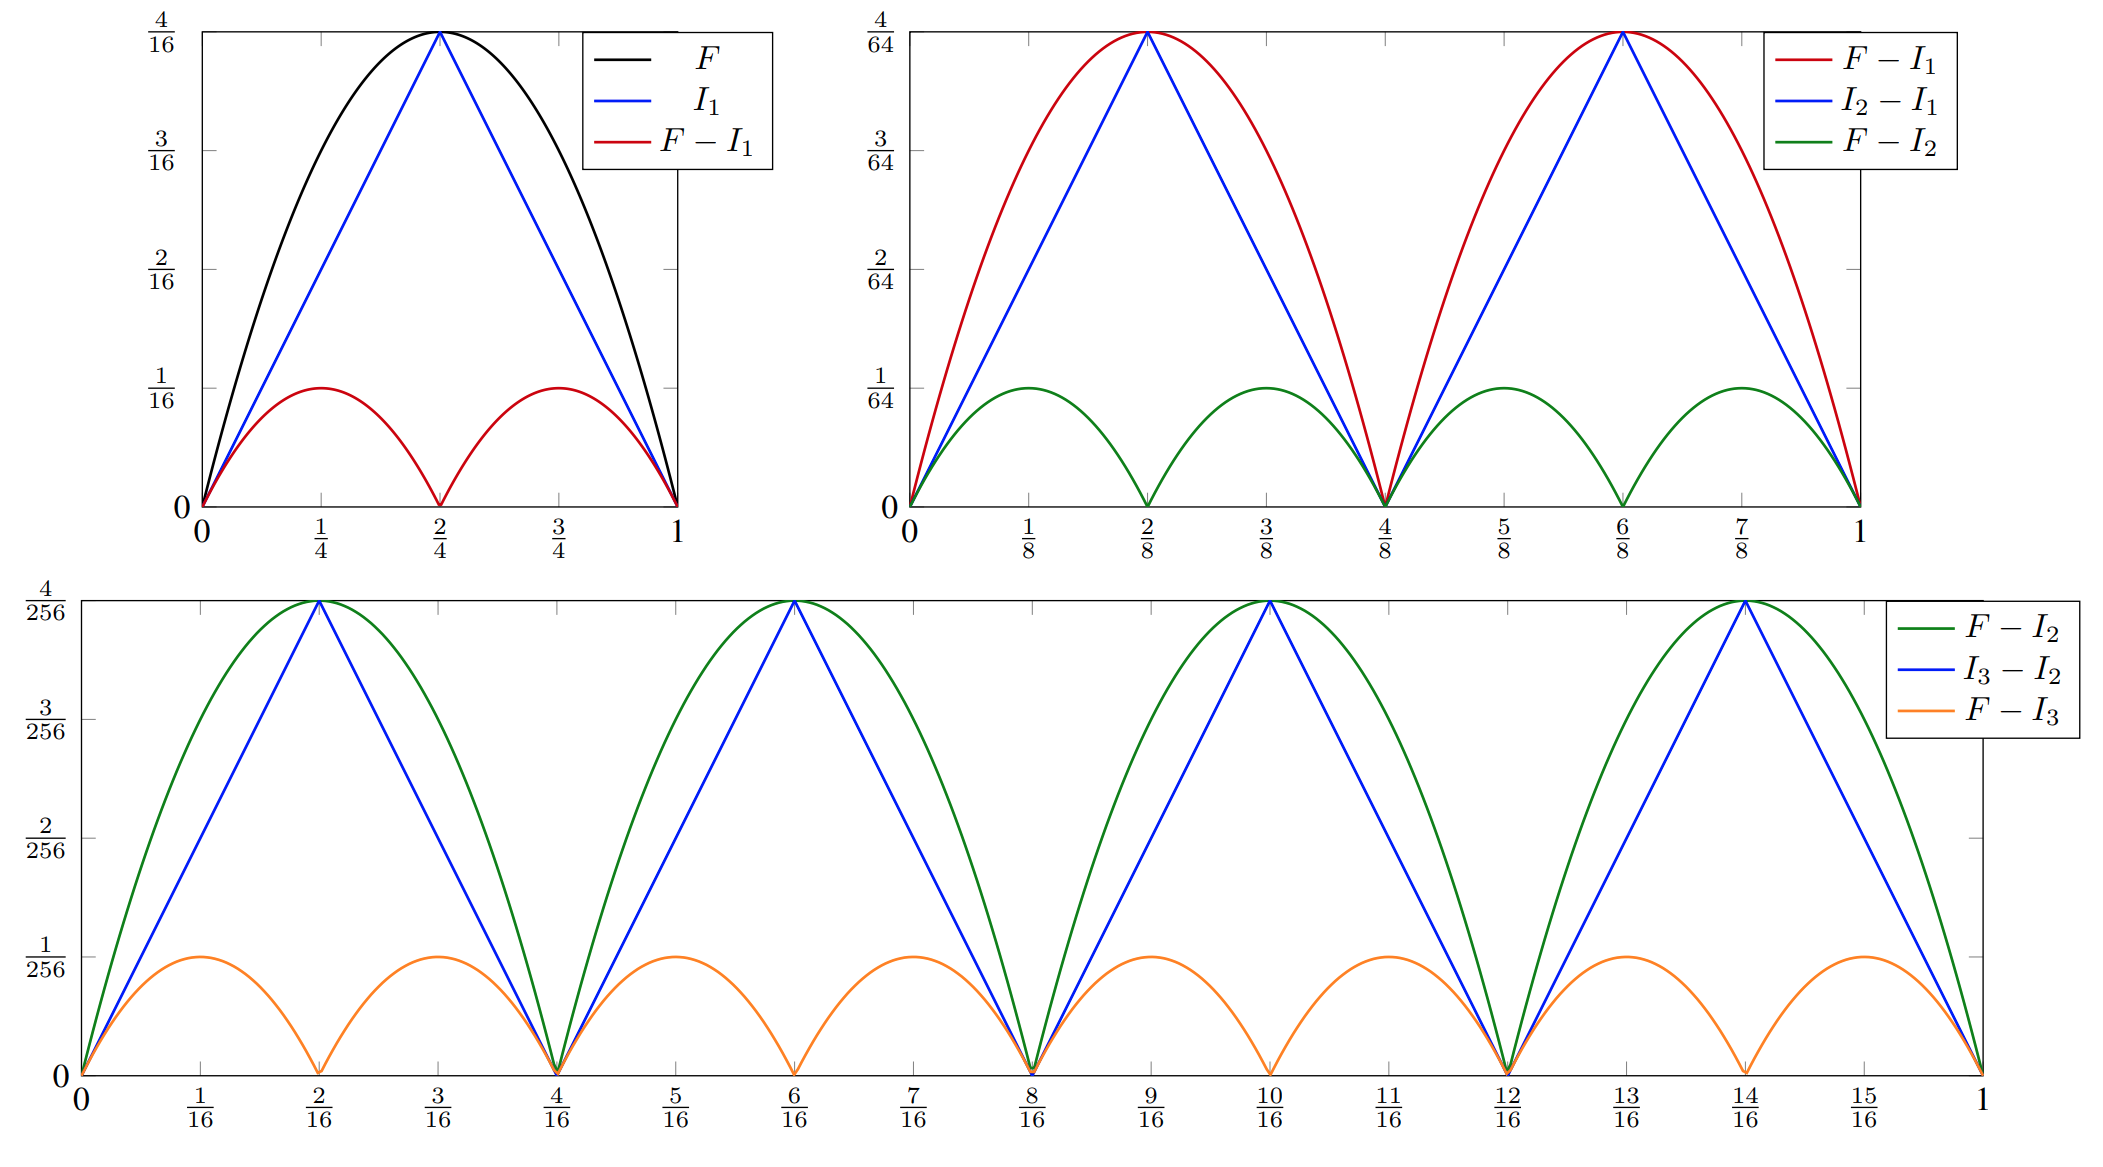
\includegraphics[height=0.9\textheight]{images/approximation-proposition-6.png}
\end{frame}

\begin{frame}{Quadrierfunktion}
    \begin{align*}
        A_1 &\coloneqq \begin{pmatrix}
            1 \\ 1 \\ 1
        \end{pmatrix}, \quad &b_1 &\coloneqq \begin{pmatrix}
            0 \\ -2^{-1} \\ 0
        \end{pmatrix}, \\
        A_l &\coloneqq \begin{pmatrix}
            2^{-1} & -1 & 0 \\ 2^{-1} & -1 & 0 \\ -2^{-1} & 1 & 1
        \end{pmatrix}, &b_l &\coloneqq \begin{pmatrix}
            0 \\ -2^{-2l + 1} \\ 0
        \end{pmatrix}, \\
        A_{m+1} &\coloneqq (-2^{-1}, 1, 1), \quad &b_{m+1} &\coloneqq 0
    \end{align*}
\end{frame}

\subsection{Multiplikationsfunktion}

\begin{frame}{Multiplikationsfunktion}
    \begin{proposition} % iii.3
        Es existiert eine Konstante \(C>0\), sodass für alle \(D\in \R_+\) und \(\varepsilon \in (0, 1/2)\) 
        ein Netzwerk \(\Phi_{D,\varepsilon} \in \mathcal{N}_{2,1}\) existiert mit 
        \(\mathcal{L}(\Phi_{D, \varepsilon}) \leq C (\log(\lceil D \rceil) + \log(\varepsilon^{-1})) \), 
        \(\mathcal{W}(\Phi_{D, \varepsilon}) \leq 5\), \(\mathcal{B}(\Phi_{D, \varepsilon}) = 1\) sowie 
        \(\Phi_{D,\varepsilon}(0,x) = \Phi_{D,\varepsilon}(x,0) = 0 \;\forall x\in \R\) und 
        \[ \norm{\Phi_{D,\varepsilon}(x,y) - xy}_{L^\infty([-D,D]^2)} \leq \varepsilon. \]
    \end{proposition}
\end{frame}

\begin{frame}{Multiplikationsfunktion}
    \begin{align*}
        A_1 &\coloneqq \frac{1}{2D} \begin{pmatrix}
            1 & 1 \\ -1 & -1 \\ 1 & -1 \\ -1 & 1
        \end{pmatrix}, \quad b_1 \coloneqq \begin{pmatrix}
            0 \\ 0 \\ 0 \\ 0
        \end{pmatrix}, \qquad
        A_2 \coloneqq \begin{pmatrix}
            1 & 1 & 0 & 0 \\
            1 & 1 & 0 & 0 \\
            1 & 1 & -1 & -1 \\
            0 & 0 & 1 & 1 \\
            0 & 0 & 1 & 1
        \end{pmatrix}, \quad b_2 \coloneqq \begin{pmatrix}
            0 \\ -2^{-1} \\ 0 \\ 0 \\ -2^{-1}
        \end{pmatrix} \\
        A_l &\coloneqq \begin{pmatrix}
            2^{-1} & -1 & 0 & 0 & 0 \\
            2^{-1} & -1 & 0 & 0 & 0 \\
            -2^{-1} & 1 & 1 & 2^{-1} & -1 \\
            0 & 0 & 0 & 2^{-1} & -1 \\
            0 & 0 & 0 & 2^{-1} & -1
        \end{pmatrix}, \quad b_l \coloneqq \begin{pmatrix}
            0 \\ -2^{-2l+3} \\ 0 \\ 0 \\ -2^{-2l+3}
        \end{pmatrix}, \text{ für } l \in \set{3, \ldots, m+1} \\
        A_{m+2} &\coloneqq \begin{pmatrix}
            -2^{-1} & 1 & 1 & 2^{-1} & -1
        \end{pmatrix}, \quad b_{m+2} \coloneqq 0
    \end{align*}
\end{frame}

\subsection{Polynome}

\begin{frame}{Polynome}
    \begin{proposition} % iii.5
        \newcommand{\Phia}{\Phi_{a,D,\varepsilon}}
        Es existiert eine Konstante \(C>0\), sodass für alle \(m\in \N\), \(a = (a_i)_{i=0}^m \in \R^{m+1}\), 
        \(D\in \R_+\) und \(\varepsilon \in (0,1/2)\) ein Netzwerk \(\Phia \in \mathcal{N}_{1,1}\) 
        existiert mit \(\mathcal{L}(\Phia) \leq C m (\log(\varepsilon^{-1}) + m\log(\lceil D \rceil) + \log(m) + \log(\lceil \norm{a}_\infty \rceil))\), 
        \(\mathcal{W}(\Phia) \leq 9\), \(\mathcal{B}(\Phia) \leq 1\) sowie 
        \[ \left\|\Phia(x) - \sum_{i=0}^m a_i x^i \right\|_{L^\infty([-D,D])} \leq \varepsilon. \]
    \end{proposition}
\end{frame}

\subsection{Glatte Funktionen}

\begin{frame}{Approximationssatz von Weierstrass}
    \begin{satz*}[Approximationssatz von Weierstrass] % iii.6
        Sei \([a,b] \subset \R\) und \(f\in C([a,b])\). Dann existiert für jedes \(\varepsilon > 0\) ein 
        Polynom \(\pi\), sodass 
        \[ \norm{f - \pi }_{L^\infty([a,b])} \leq \varepsilon. \]
    \end{satz*}
\end{frame}

\begin{frame}{Glatte Funktionen}
    \begin{lemma} % iii.7
        Betrachte die Menge der Funktionen 
        \[ \mathcal{S}_{[-1,1]} \coloneqq \left\{ f \in C^\infty([-1,1], \R): \norm{f^{(n)}}_{L^\infty([-1,1])} \leq n! \;\forall n \in \N_0 \right\}. \]
        Dann existiert eine Konstante \(C>0\), sodass für alle \(f\in \mathcal{S}_{[-1,1]}\) und \(\varepsilon\in (0,1/2)\) 
        ein Netz \(\Psi_{f,\varepsilon} \in \mathcal{N}_{1,1}\) existiert mit 
        \( \mathcal{L}(\Psi_{f,\varepsilon}) \leq C(\log(\varepsilon^{-1}))^2 \), 
        \(\mathcal{W}(\Psi_{f,\varepsilon}) \leq 9\), \(\mathcal{B}(\Psi_{f,\varepsilon}) \leq 1\) 
        sowie 
        \[ \norm{\Psi_{f,\varepsilon} - f}_{L^\infty([-1,1])} \leq \varepsilon. \]
    \end{lemma}
\end{frame}

\subsection{Trigonometrische Funktionen}

\begin{frame}{Trigonometrische Funktionen}
    \begin{satz} % iii.8
        \newcommand{\Psia}{\Psi_{a,D,\varepsilon}}
        Es existiert eine Konstante \(C>0\), sodass für alle \(a,D\in \R_+\), \(\varepsilon \in (0,1/2)\) 
        ein Netzwerk \(\Psia \in \mathcal{N}_{1,1}\) mit \(\mathcal{L}(\Psia) \leq C((\log(\varepsilon^{-1}))^2 + \log(\lceil aD\rceil))\), 
        \(\mathcal{W}(\Psia) \leq 9\), \(\mathcal{B}(\Psia) \leq 1\) sowie 
        \[ \norm{\Psia - \cos(a x) }_{L^{\infty}([-D,D])} \leq \varepsilon. \]
    \end{satz}
\end{frame}

\begin{frame}{Trigonometrische Funktionen}
    \begin{korollar} % iii.9
        \newcommand{\Psia}{\Psi_{a,b,D,\varepsilon}}
        Es existiert eine Konstante \(C>0\), sodass für alle \(a,D\in \R_+\), \(b\in \R\), \(\varepsilon \in (0,1/2)\) 
        ein Netzwerk \(\Psia \in \mathcal{N}_{1,1} \) mit 
        \(\mathcal{L}(\Psia) \leq C((\log(\varepsilon^{-1}))^2 + \log(\lceil a D + |b| \rceil))\), 
        \(\mathcal{W}(\Psia) \leq 9\), \(\mathcal{B}(\Psia) \leq 1\) sowie 
        \[ \norm{\Psia - \cos(a x - b) }_{L^\infty([-D,D])} \leq \varepsilon \text{ existiert}. \]
    \end{korollar}
\end{frame}

\begin{frame}{Abschluss} % iii.10
    \begin{itemize}
        \item Netzwerke mit endlicher Breite und Tiefe, die polylogarithmisch in \(\varepsilon^{-1}\) wächst, können die Funktionenklassen approximieren \pause
        \item Wegen \(\mathcal{M}(\Phi) \leq \mathcal{L}(\Phi) \mathcal{W}(\Phi)(\mathcal{W}(\Phi) + 1)\) wächst die Konnektivität auch nur polylogarithmisch in \(\varepsilon^{-1}\) \pause
        \item \( \Rightarrow \) der Approximationsfehler \(\varepsilon\) fällt exponentiell in der Konnektivität/der Anzahl der Parametern im neuronalen Netz
    \end{itemize}
\end{frame}

\begin{frame}{Referenzen}
    \footnotesize
    \nocite{Grohs2019}
    \printbibliography[heading=none]
\end{frame}

\end{document}